\documentclass[12pt, a4paper]{article}
\usepackage[utf8]{inputenc}
\usepackage[T1]{fontenc}
\usepackage[brazil]{babel}
\usepackage{graphicx}
\usepackage[font=footnotesize, labelfont=bf, listformat=empty]{caption}
\usepackage{setspace}
\usepackage{indentfirst}
\usepackage{geometry}
\usepackage{listings}
\usepackage{titlesec}
\usepackage{fancyhdr}
\usepackage{lastpage}
\usepackage{dirtree}
\usepackage{amsmath}
\usepackage{mdframed}
\usepackage{amssymb}
\usepackage[colorlinks=true, allcolors=black]{hyperref}
\usepackage{tikz, tkz-base, tkz-fct}
\usepackage{fix-cm}
\usepackage{lmodern}
\usepackage{shadowtext}
\usepackage{minted}

% Configurações de listagens
\renewcommand{\listingscaption}{Código}
\newenvironment{code}{\captionsetup{type=listing}}{}


% Configurações de margens e espaçamento
\geometry{a4paper, left=3cm, right=2cm, top=3cm, bottom=2cm}
\setlength{\parindent}{1.25cm}
\onehalfspacing

% Configurações de cabeçalho e rodapé
\pagestyle{fancy}
\fancyhf{}
\fancyhead[L]{\footnotesize{SimulNet - Projeto de TR1}}
\fancyhead[R]{\footnotesize{\thepage\ de \pageref{LastPage}}}
\fancyfoot[C]{\footnotesize{Relatório de Implementação do SimulNet}}

% Configurações de títulos
\titleformat{\section}{\normalfont\large\bfseries}{\thesection}{1em}{}
\titleformat{\subsection}{\normalfont\bfseries}{\thesubsection}{1em}{}
\titleformat{\subsubsection}{\normalfont\itshape}{\thesubsubsection}{1em}{}

% Definindo cores personalizadas
\definecolor{roxo}{RGB}{128, 0, 128} % Roxo
\definecolor{verde}{RGB}{0, 128, 0} % Verde
\definecolor{cinza_claro}{RGB}{240, 240, 240} % Cinza claro
\definecolor{verde_claro}{RGB}{124, 200, 66} % Verde claro

\begin{document}

% Capa
\begin{titlepage}
    \tikz[remember picture,overlay] \node[opacity=1.0,inner sep=0pt] at (current page.center){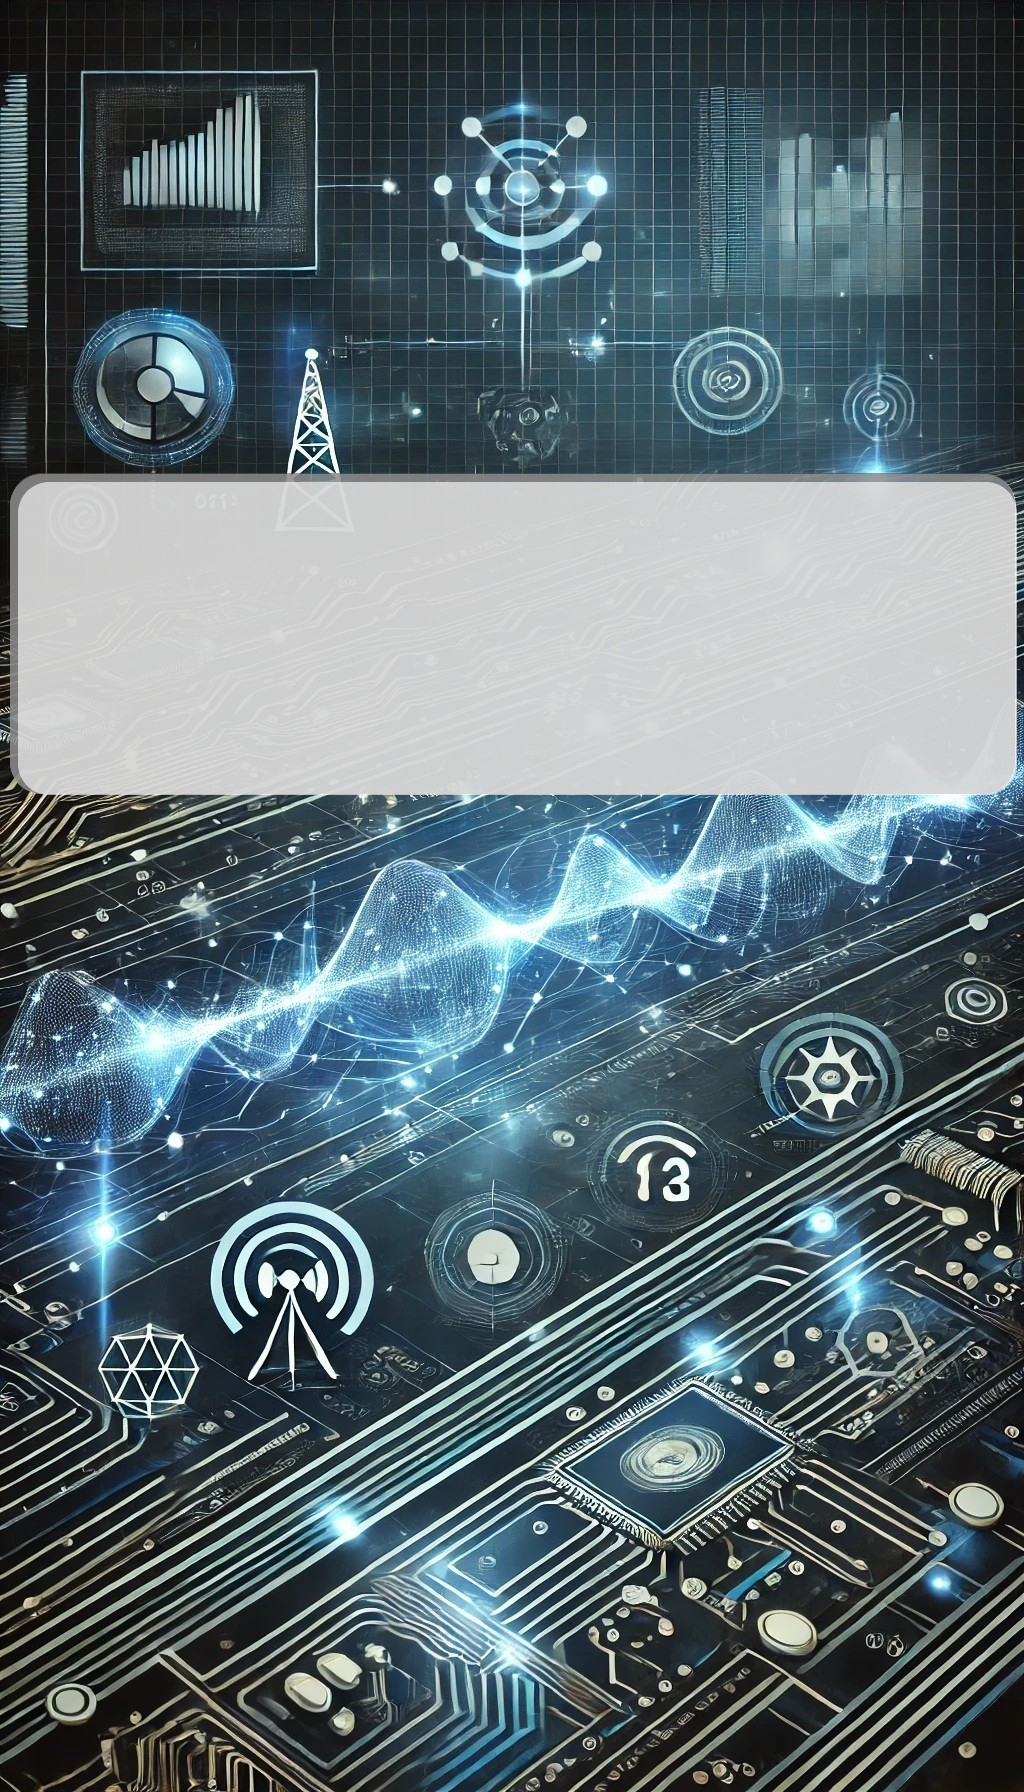
\includegraphics[width=\paperwidth,height=\paperheight]{image/Capa_TR1_v1.jpg}};
    \begin{center}
        \vspace*{5cm} % Espaço no topo para o título
        \shadowcolor{white}
        {\fontsize{46}{51}\selectfont \textbf{SimulNet}} \\ % Título grande
        \vspace{1.5cm} % Espaço entre o título e o nome do autor
        \shadowcolor{gray}
        {\fontsize{20}{25}\selectfont Henrique Morcelles Salum} \\ % Nome do autor
        {\fontsize{15}{20}\selectfont 232003008} \\ % Número de identificação
        \vfill
    \end{center}
\end{titlepage}

% Sumário
\tableofcontents
\newpage

% Introdução
\section{Introdução}
\paragraph{}
O modelo OSI (Open Systems Interconnection) é um modelo de referência que descreve as funções de comunicação em redes de computadores. O modelo é dividido em sete camadas, cada uma responsável por funções específicas que garantem a comunicação eficiente entre dispositivos.

\begin{figure}[h]
    \centering
    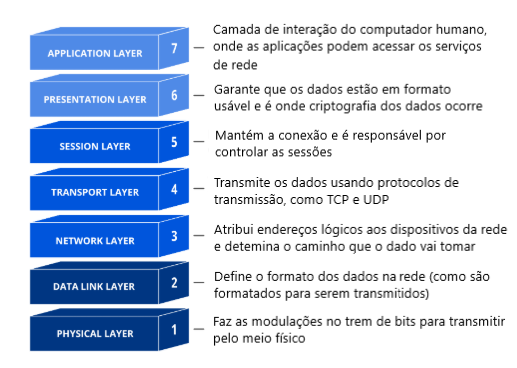
\includegraphics[width=0.5\textwidth]{image/Modelo_Osi.png}
    \caption{Modelo OSI de sete camadas.}
\end{figure}

\paragraph{}
Este relatório descreve a implementação de um simulador que aborda as camadas física e de enlace do modelo OSI. O objetivo principal é simular o funcionamento dessas camadas, incluindo técnicas de modulação digital - NRZ-Polar, Manchester e Bipolar, modulação por portadora - ASK, FSK e 8-QAM, enquadramento de dados - Contagem de Caracteres e Inserção de Bytes, detecção e correção de erros - Bit de Paridade, Código de Redundância Cíclica (CRC) e Código de Hamming. O simulador foi desenvolvido em Python, proporcionando uma visão prática dos mecanismos fundamentais que garantem a transmissão eficiente e confiável de dados em redes de computadores.

\paragraph{}
O problema central a ser resolvido consiste na simulação de um sistema de comunicação que possibilite a transmissão de dados entre dois pontos, considerando os desafios inerentes à presença de ruído e erros de transmissão — simulados no projeto. O simulador deve ser capaz de transmitir e receber dados de forma confiável, aplicando técnicas de modulação, enquadramento, detecção e correção de erros. A comunicação entre os dois pontos é realizada por meio de \textit{sockets}, biblioteca da linguagem Python, onde dois processos distintos — um transmissor e um receptor — interagem para simular a troca de dados em um cenário realista.

\newpage

\subsection{Estrutura do Projeto}
\paragraph{}
O projeto está organizado em uma estrutura de diretórios que facilita a modularidade e a manutenção do código. A seguir, descrevemos a organização dos arquivos e diretórios:

\begin{figure}[ht]
    \centering
    \begin{mdframed}[
        linewidth=0pt, % Espessura da borda
        roundcorner=10pt, % Borda arredondada
        backgroundcolor=cinza_claro, % Fundo branco
        innertopmargin=10pt, % Espaçamento interno
        innerbottommargin=10pt,
        innerleftmargin=20pt,
        innerrightmargin=20pt
    ]
    \dirtree{%
    .1 \textbf{Projeto\_TR1}.
    .2 \textcolor{roxo}{gui}.
    .3 transmissor.py.
    .3 receptor.py.
    .2 \textcolor{verde}{src}.
    .3 transmissor.
    .4 \_\_init\_\_.py.
    .4 camada\_fisica.py.
    .4 camada\_enlace.py.
    .3 receptor.
    .4 \_\_init\_\_.py.
    .4 camada\_fisica.py.
    .4 camada\_enlace.py.
    .3 \textcolor{verde_claro}{utils}.
    .4 bytes\_to\_string.py.
    .4 listBool\_to\_bytes.py.
    .4 string\_to\_bytes.py.
    .4 text\_to\_bytes.py.
    }
    \end{mdframed}
    \caption{Estrutura de diretórios do projeto.}
    \label{fig:estrutura}
\end{figure}

\paragraph{}
O diretório \textcolor{roxo}{gui} contém os arquivos \textit{transmissor.py} e \textit{receptor.py}, que são responsáveis por iniciar a interface gráfica do simulador. O diretório \textcolor{verde}{src} contém os módulos \textit{transmissor} e \textit{receptor}, que implementam as funcionalidades da camada física e de enlace do modelo OSI. O diretório \textcolor{verde_claro}{utils} contém funções auxiliares que são utilizadas em diferentes partes do projeto.

\subsection{Funcionamento do Simulador}
\paragraph{}
Para utilizar o simulador, é necessário executar o arquivo \textit{transmissor.py} em um terminal e o arquivo \textit{receptor.py} em outro. O transmissor exibe uma interface gráfica que permite configurar os parâmetros de modulação por portadora — como o tamanho da amostragem, a frequência, a amplitude e a fase padrão utilizadas para gerar o sinal —, além dos parâmetros de transmissão, como a técnica de modulação, o enquadramento de dados e a detecção de erros. A interface também possibilita a visualização dos sinais gerados após cada etapa de modulação.

\paragraph{}
Por sua vez, o receptor exibe uma interface gráfica que permite visualizar o sinal recebido e a mensagem decodificada após a demodulação. Além disso, a interface do receptor conta com um botão "Abrir Servidor", que habilita o transmissor a enviar os dados.

\paragraph{}
Após configurar os parâmetros no transmissor e abrir o servidor no receptor, o usuário deve clicar no botão "Enviar Dados" na interface do transmissor para iniciar a transmissão. Esse processo garante que os dados sejam enviados e recebidos corretamente, permitindo a simulação completa da comunicação entre os dois pontos.

\begin{figure}[ht]
    \centering
    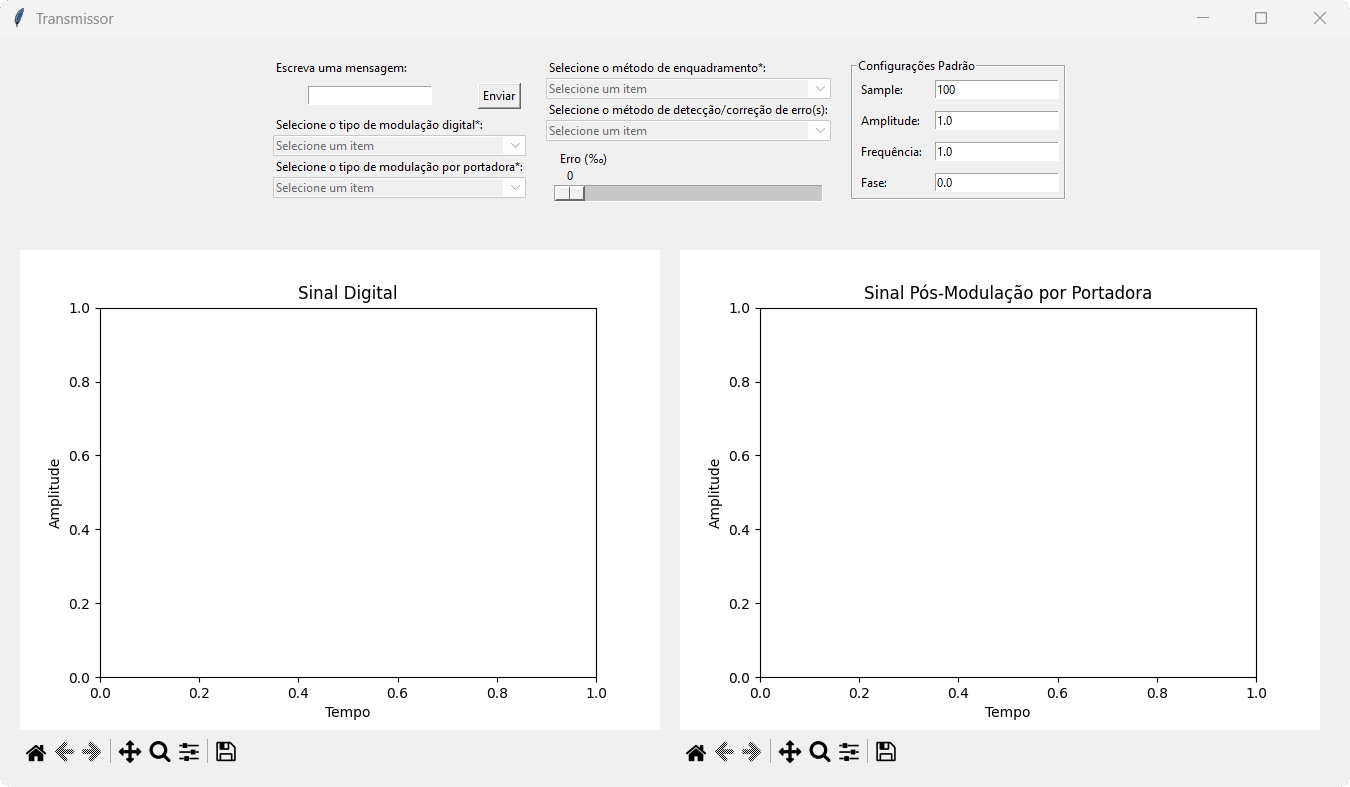
\includegraphics[width=0.8\textwidth]{image/interface_transmissor.png}
    \caption{Interface gráfica do transmissor}
\end{figure}

\begin{figure}[ht]
    \centering
    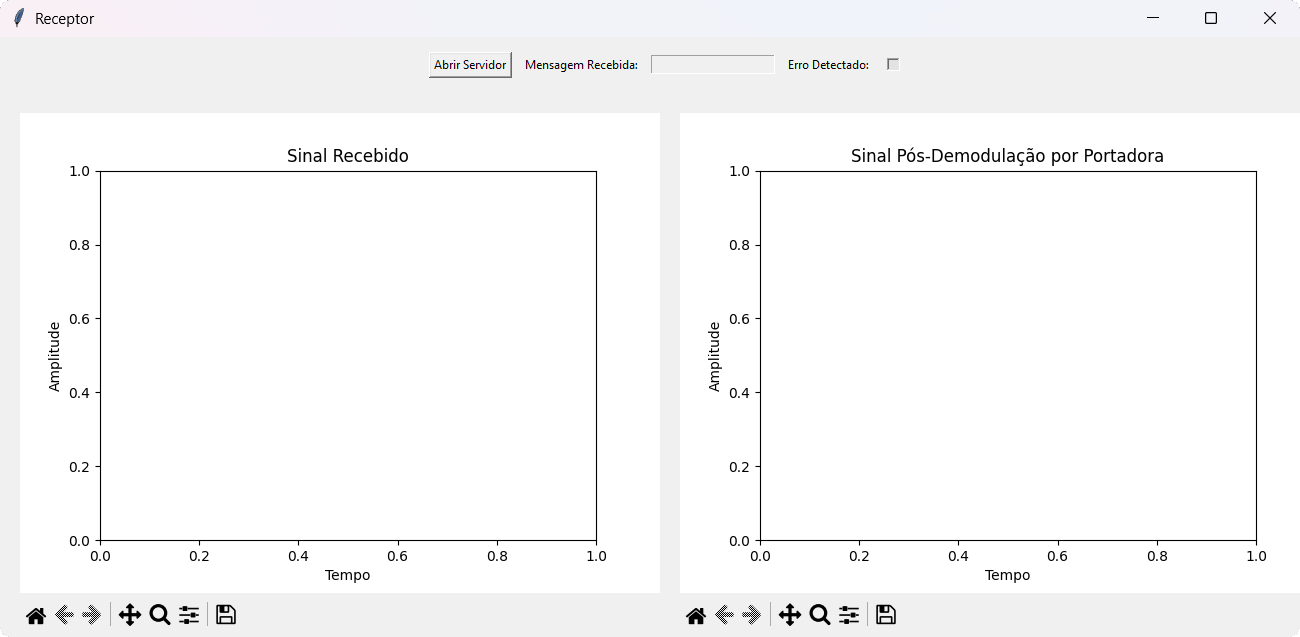
\includegraphics[width=0.8\textwidth]{image/interface_receptor.png}
    \caption{Interface gráfica do receptor}
\end{figure}

\newpage

% Implementação
\section{Implementação}
\paragraph{}
Nessa seção, apresentamos a implementação do projeto, expondo os códigos desenvolvidos para realizá-lo. Note, porém, que os códigos aqui expostos não têm comentários, isto porque, para melhor apresentação deste documento, a devida documentação foi reservada ao projeto em si, sendo ocultada aqui.

\subsection{Transmissor}

\subsubsection{Camada Física}
\paragraph{}
A camada física do transmissor é responsável por gerar o sinal modulado a partir da mensagem de entrada. Foram implementadas as técnicas de modulação NRZ-Polar, Manchester, Bipolar, ASK, FSK e 8-QAM.

\begin{code}
\begin{minted}[breaklines=true, breakanywhere=true, linenos=true, bgcolor=cinza_claro]{python}
from math import sin, cos, ceil, pi

class CamadaFisicaTransmissor:
    def __init__(self, sample: int = 100, frequencia: float = 1.0, amplitude: float = 1.0, fase: float = 1.0) -> None:
        self.sample: int = sample
        self.frequencia: float = frequencia
        self.amplitude: float = amplitude
        self.fase: float = fase

    def gerador_bit_stream(self, mensagem: str) -> list[bool]:
        return [True if char == '1' else False for char in mensagem]

    # Modulação Digital
    def nrz_polar(self, bit_stream: list[bool]) -> list[int]:
        return [1 if bit else -1 for bit in bit_stream]

    def manchester(self, bit_stream: list[bool]) -> list[int]:
        i: int = 0
        clk: bool = 0
        dig_signal: list[int] = []

        while i < len(bit_stream):
            dig_signal.append(int(bit_stream[i] ^ clk))
            i += 1 * clk
            clk = not clk
        return dig_signal

    def bipolar(self, bit_stream: list[bool]) -> list[int]:
        last_one: int = 1
        dig_signal: list[int] = []

        for bit in bit_stream:
            if not bit:
                dig_signal.append(0)
            else:
                last_one = -last_one
                dig_signal.append(last_one)
        return dig_signal

    # Modulação por portadora
    def ask(self, dig_signal: list[int], mod_digital: str, amp_zero: int = 0, amp_one: int = 1) -> list[float]:
        signal: list[float] = [0.0] * (len(dig_signal) * self.sample)
        nrz_polar: bool = mod_digital == "NRZ-Polar"

        for i in range(len(dig_signal)):
            for j in range(self.sample):
                t: float = j / self.sample
                if ((dig_signal[i] == 1 or dig_signal == -1) and not nrz_polar) or dig_signal[i] == 1:
                    signal[i * self.sample + j] = amp_one * sin(2*pi*self.frequencia*t + self.fase)
                else:
                    signal[i * self.sample + j] = amp_zero * sin(2*pi*self.frequencia*t + self.fase)
        return signal

    def fsk(self, dig_signal: list[int], mod_digital: str, f_zero: float = 0.0, f_one: float = 1.0) -> list[float]:
        signal: list[float] = [0.0] * (len(dig_signal) * self.sample)
        nrz_polar: bool = mod_digital == "NRZ-Polar"

        for i in range(len(dig_signal)):
            for j in range(self.sample):
                t: float = j / self.sample
                if ((dig_signal[i] == 1 or dig_signal == -1) and not nrz_polar) or dig_signal[i] == 1:
                    signal[i * self.sample + j] = self.amplitude * sin(2*pi*f_one*t + self.fase)
                else:
                    signal[i * self.sample + j] = self.amplitude * sin(2*pi*f_zero*t + self.fase)
        return signal

    def qam8_modulation(self, dig_signal: list[int], mod_digital: str) -> list[float]:
        signal: list[float] = [0.0] * (ceil(len(dig_signal) / 3) * self.sample)
        constellation: dict[str, complex] = {
            "000": 1 + 1j, "001": 1 - 1j, "010": -1 + 1j,
            "011": -1 - 1j, "100": 1/3 + 1/3j, "101": 1/3 - 1/3j,
            "110": -1/3 + 1/3j, "111": -1/3 - 1/3j
        }

        while len(dig_signal) % 3:
            dig_signal.insert(0, 0)

        if mod_digital == "NRZ-Polar":
            bit_stream: str = ''.join('1' if elemento == 1 else '0' for elemento in dig_signal)
        elif mod_digital == "Bipolar":
            bit_stream: str = ''.join('1' if abs(elemento) == 1 else '0' for elemento in dig_signal)
        else: 
            bit_stream: str = ''.join('1' if elemento == 1 else '0' for elemento in dig_signal)
        symbols: list[complex] = [constellation[bit_stream[i:i + 3]] for i in range(0, len(bit_stream), 3)]

        for i in range(len(symbols)):
            for j in range(self.sample):
                t: float = j / self.sample
                signal[i * self.sample + j] = symbols[i].real * cos(2*pi*self.frequencia*t) + symbols[i].imag * sin(2*pi*self.frequencia*t)
        return signal
\end{minted}
\caption{Implementação da camada física do transmissor}
\end{code}

\subsubsection{Camada de Enlace}
\paragraph{}
A camada de enlace foi implementada com foco em enquadramento de dados, detecção de erros e correção de erros. Foram utilizados métodos de enquadramento por contagem de caracteres e inserção de bytes. Para detecção de erros, foram implementados o bit de paridade par e o CRC-32. Para correção de erros, foi utilizado o código de Hamming.

\begin{code}
\begin{minted}[breaklines=true, breakanywhere=true, linenos=true, bgcolor=cinza_claro]{python}
from math import log2

class CamadaEnlaceTransmissor:
    def __init__(self) -> None:
        self.FLAG: bytes = bytes([22])
        self.ESC: bytes = bytes([27])
        self.CRC32_POLY: int = 0x04C11DB7
    
    def contagem_de_caracteres(self, byte_stream: bytes, maxFrameSize: int = 4) -> bytes:
        frames: bytearray = bytearray()
        while byte_stream:
            frame: bytes = byte_stream[:maxFrameSize]
            byte_stream = byte_stream[maxFrameSize:]
            frames.append(len(frame))
            frames.extend(frame)
        return bytes(frames)
    
    def insercao_de_bytes(self, byte_stream: bytes, maxFrameSize: int = 4) -> bytes:
        frames: bytearray = bytearray()
        while byte_stream:
            frames.extend(self.FLAG)
            i: int = 0
            while i < maxFrameSize and byte_stream:
                if byte_stream[:1] == self.FLAG or byte_stream[:1] == self.ESC:
                    frames.extend(self.ESC)
                frames.extend(byte_stream[:1])
                byte_stream = byte_stream[1:]
                i += 1
            frames.extend(self.FLAG)
        return bytes(frames)
    
    def bit_de_paridade(self, byte_stream: bytes) -> str:
        bit_stream: list[int] = [int(x) for x in ''.join(f'{byte:08b}' for byte in byte_stream)] + [0]
        for bit in bit_stream[:-1]:
            bit_stream[-1] ^= bit
        return ''.join(str(bit) for bit in bit_stream)
    
    def crc32(self, byte_stream: bytes) -> str:
        bit_stream: str = ''.join(f'{byte:08b}' for byte in byte_stream)
        crc: int = int.from_bytes(byte_stream, byteorder="big") << 32
        while crc.bit_length() >= 32:
            bytes_a_processar = (crc >> (crc.bit_length() - 32)) & 0xFFFFFFFF
            if bytes_a_processar & 0x80000000:
                bytes_a_processar ^= self.CRC32_POLY
            else:
                bytes_a_processar ^= 0
            crc = ((bytes_a_processar & 0x7FFFFFFF) << (crc.bit_length() - 32)) | (crc & ((1 << (crc.bit_length() - 32)) - 1))
        return bit_stream + f"{crc:032b}"
    
    def hamming(self, byte_stream: bytes) -> str:
        bit_stream: list[int] = [int(bit) for byte in byte_stream for bit in f'{byte:08b}']
        m: int = len(bit_stream)
        r: int = 0
        while (2**r) < (m + r + 1):
            r += 1
        hamming_code: list[int] = []
        j = 0
        for i in range(1, m + r + 1):
            if log2(i).is_integer():
                hamming_code.append(0)
            else:
                hamming_code.append(bit_stream[j])
                j += 1
        for i in range(r):
            pos = 2**i
            paridade = 0
            for j in range(1, len(hamming_code) + 1):
                if j & pos:
                    paridade ^= hamming_code[j - 1]
            hamming_code[pos - 1] = paridade
        return ''.join(str(bit) for bit in hamming_code)
\end{minted}
\caption{Implementação da camada de enlace do transmissor}
\end{code}

\subsection{Receptor}

\subsubsection{Camada Física}
\paragraph{}
A camada física do receptor é responsável por demodular o sinal recebido e extrair o trem de bits transmitido. Foram implementadas as técnicas de demodulação NRZ-Polar, Manchester, Bipolar, ASK e FSK. Perceba que a decodificação 8-QAM não foi implementada. Isso se deve ao imenso trabalho que tentar implementá-la gerou, mesmo sem sucesso. A forma como é enviada a mensagem caso seja escolhida a modulação 8-QAM será explicada doravante.

\begin{code}
\begin{minted}[breaklines=true, breakanywhere=true, linenos=true, bgcolor=cinza_claro]{python}
from math import cos, sin, pi

class CamadaFisicaReceptor:
    def __init__(self, sample, amplitude, frequencia, fase) -> None:
        self.sample = sample
        self.amplitude = amplitude
        self.frequencia = frequencia
        self.fase = fase
    
    def decodificar_nrz_polar(self, dig_signal: list[int]) -> list[bool]:
        return [False if bit == -1 else True for bit in dig_signal]
    
    def decodificar_manchester(self, dig_signal: list[int]) -> list[bool]:
        bit_stream: list[bool] = []
        i: int = 0
        while i < len(dig_signal):
            bit_stream.append(True if dig_signal[i] == 1 else False)
            i += 2
        return bit_stream
    
    def decodificar_bipolar(self, dig_signal: list[int]) -> list[bool]:
        return [False if bit == 0 else True for bit in dig_signal]
    
    def decodificar_ask(self, signal: list[float], mod_digital: str, amp_zero: float = 0, amp_one: float = 1) -> list[int]:
        if mod_digital == "NRZ-Polar":
            return [1 if max(signal[i:i+self.sample]) > (amp_zero + amp_one) / 2 else -1 for i in range(0, len(signal), self.sample)]
        elif mod_digital == "Bipolar":
            dig_signal: list[int] = []
            last_one = -1
            for i in range(0, len(signal), self.sample):
                if (max(signal[i:i+self.sample]) - amp_zero) > (max(signal[i:i+self.sample]) - amp_one):
                    last_one = -last_one
                    dig_signal.append(last_one)
                else:
                    dig_signal.append(0)
            return dig_signal
        else:
            return [1 if (max(signal[i:i+self.sample]) - amp_zero) > (max(signal[i:i+self.sample]) - amp_one) else 0 for i in range(0, len(signal), self.sample)]
    
    def decodificar_fsk(self, mod_signal: list[float], mod_digital: str, f_zero: float = 0.0, f_one: float = 1.0) -> list[int]:
        bit_stream: list[int] = []
        for i in range(0, len(mod_signal), self.sample):
            janela: list[float] = mod_signal[i:i + self.sample]
            cruzamentos: int = 0
            for j in range(1, len(janela)):
                if (janela[j-1] < 0 and janela[j] > 0) or (janela[j-1] > 0 and janela[j] < 0):
                    cruzamentos += 1
            if mod_digital == "NRZ-Polar":
                bit_stream.append(-1 if abs(cruzamentos - f_zero) < abs(cruzamentos - f_one) else 1)
            elif mod_digital == "Bipolar":
                last_one = -1
                if abs(cruzamentos - f_zero) > abs(cruzamentos - f_one):
                    last_one = -last_one
                    bit_stream.append(last_one)
                else:
                    bit_stream.append(0)
            else:
                bit_stream.append(0 if abs(cruzamentos - f_zero) < abs(cruzamentos - f_one) else 1)
        return bit_stream
\end{minted}
\caption{Implementação da camada física do receptor}
\end{code}

\subsubsection{Camada de Enlace}
\paragraph{}
A camada de enlace do receptor é responsável por extrair a mensagem transmitida a partir do trem de bits recebido. Foram implementados os métodos de desenquadramento por contagem de caracteres e inserção de bytes, além da detecção e correção de erros por bit de paridade, CRC-32 e código de Hamming.

\begin{code}
\begin{minted}[breaklines=true, breakanywhere=true, linenos=true, bgcolor=cinza_claro]{python}
from math import log2
from src.utils import bytes_to_string

class CamadaEnlaceReceptor:
    def __init__(self):
        self.FLAG: bytes = bytes([22])
        self.ESC: bytes = bytes([27])
        self.CRC32_POLY = 0x04C11DB7

    def desenquadramento_contagem_de_caracteres(self, byte_stream: bytes) -> bytes:
        pacote: bytearray = bytearray()
        while byte_stream:
            length: int = int(byte_stream[0])
            byte_stream = byte_stream[1:]
            frame = byte_stream[:length]
            byte_stream = byte_stream[length:]
            pacote.extend(frame)
        return bytes(pacote)
    
    def desenquadramento_insercao_de_bytes(self, byte_stream: bytes) -> bytes:
        pacote: bytearray = bytearray()
        esc: bool = False
        while byte_stream:
            byte_atual = byte_stream[:1]
            byte_stream = byte_stream[1:]
            
            if byte_atual == self.FLAG and not esc:
                continue
            elif byte_atual == self.ESC and not esc:
                esc = True
                continue
            else:
                pacote.extend(byte_atual)
                esc = False
            
        return bytes(pacote)

    def verificar_bits_de_paridade(self, byte_stream: bytes) -> tuple[bytes, bool]:
        bit_stream: list[int] = [int(x) for x in bytes_to_string(byte_stream)]
        paridade = 0
        bit_stream_util = bit_stream[:-1]
        for bit in bit_stream_util:
            paridade ^= bit
            
        byte_stream_saida = bytes(int("".join(str(bit) for bit in bit_stream_util[i:i+8]), 2)   for i in range(0, len(bit_stream_util), 8))
        
        return byte_stream_saida, paridade == bit_stream[-1]
        
    def verificar_crc32(self, byte_stream: bytes) -> tuple[bytes, bool]:
        crc_recebido: int = int.from_bytes(byte_stream[-4:], byteorder="big")
        byte_stream = byte_stream[:-4]

        crc_calculado: int = int.from_bytes(byte_stream, byteorder="big") << 32
        
        while crc_calculado.bit_length() >= 32:
            bytes_a_processar = (crc_calculado >> (crc_calculado.bit_length() - 32)) & 0xFFFFFFFF  
            if bytes_a_processar & 0x80000000:
                bytes_a_processar ^= self.CRC32_POLY
            else:
                bytes_a_processar ^= 0
            crc_calculado = ((bytes_a_processar & 0x7FFFFFFF) << (crc_calculado.bit_length() - 32)) | (crc_calculado & ((1 << (crc_calculado.bit_length() - 32)) - 1))

        return byte_stream, crc_calculado == crc_recebido

    def corrigir_hamming(self, encoded_bytes: bytes) -> tuple[bytes, bool]:
        hamming_code: list[int] = [int(bit) for bit in ''.join(f'{byte:08b}' for byte in encoded_bytes)]
        
        r: int = 0
        n: int = len(hamming_code)
        
        while (2**r) < n + 1:
            r += 1
        
        error_position = 0
        for i in range(r):
            pos = 2**i
            paridade = 0
            for j in range(n):
                if j + 1 & pos:
                    paridade ^= hamming_code[j]
            if paridade != 0:
                error_position += pos - 1
        
        error_detected = error_position != 0
        if error_detected:
            hamming_code[error_position] ^= 1
        
        original_bits = []
        for i in range(1, n + 1):
            if not log2(i).is_integer():
                original_bits.append(str(hamming_code[i - 1]))
        
        decoded_bits = ''.join(original_bits)
        decoded_bytes = bytes(int(decoded_bits[i:i+8], 2) for i in range(0, len(decoded_bits), 8))
        
        return decoded_bytes, error_detected
\end{minted}
\caption{Implementação da camada de enlace do receptor}
\end{code}

\subsection{Interface Gráfica do Transmissor}
\paragraph{}
A implementação da interface gráfica é demasiado grande e, em sua maioria, irrelevante para os propósitos deste documento. Por conseguinte, aqui serão apenas apresentadas as partes relevantes dessa implementação.

\subsubsection{Envio da Mensagem}
\paragraph{}
Essa função é responsável por recuperar os dados inseridos pelo usuário na interface gráfica e executar as funções solicitadas por ele. Note que é enviada para a função \textit{enviar\_para\_o\_receptor}, além do sinal analógico, um sinal digital. Isso será explicado adiante.

\begin{code}
\begin{minted}[breaklines=true, breakanywhere=true, linenos=true, bgcolor=cinza_claro]{python}
def enviar_mensagem(self):
    self.Bitstream = string_to_byte_stream(self.text_mensagem.get())
    self.err_value = self.sliderErr.get()
    self.mod_digital = self.select_mod_digital.get()
    self.mod_portadora = self.select_mod_portadora.get()
    self.metodo_enquadramento = self.select_enquadramento.get()
    self.metodo_deteccao_ou_correcao = self.select_detecção.get()
    self.sample = int(self.txt_sample.get())
    self.frequencia = float(self.text_frequencia.get())
    self.amplitude = float(self.text_amplitude.get())
    self.fase = float(self.text_fase.get())
    self.Fisica = CamadaFisicaTransmissor(self.sample, self.frequencia, self.amplitude, self.fase)
    self.Enlace = CamadaEnlaceTransmissor()
    
    byte_stream: bytes = bytes()
    if self.metodo_enquadramento == "Contagem de Caracteres":
        byte_stream = self.Enlace.contagem_de_caracteres(self.Bitstream)
    elif self.metodo_enquadramento == "Insercao de Bytes":
        byte_stream = self.Enlace.insercao_de_bytes(self.Bitstream)
    
    if self.metodo_deteccao_ou_correcao == "Bit de Paridade":
        byte_stream = self.Enlace.bit_de_paridade(byte_stream)
    elif self.metodo_deteccao_ou_correcao == "CRC-32":
        byte_stream = self.Enlace.crc32(byte_stream)
    elif self.metodo_deteccao_ou_correcao == "Codigo de Hamming":
        byte_stream = self.Enlace.hamming(byte_stream)
    else:
        byte_stream = bytes_to_string(byte_stream)
    
    bit_stream: list[bool] = self.Fisica.gerador_bit_stream(byte_stream)
    bit_stream_para_enviar = self.inserir_error(bit_stream.copy())
    
    dig_signal: list[int] = []
    
    if self.mod_digital == "NRZ-Polar":
        dig_signal = self.Fisica.nrz_polar(bit_stream)
        dig_signal_para_enviar = self.Fisica.nrz_polar(bit_stream_para_enviar)
    elif self.mod_digital == "Manchester":
        dig_signal = self.Fisica.manchester(bit_stream)
        dig_signal_para_enviar = self.Fisica.manchester(bit_stream_para_enviar)
    elif self.mod_digital == "Bipolar": 
        dig_signal = self.Fisica.bipolar(bit_stream)
        dig_signal_para_enviar = self.Fisica.bipolar(bit_stream_para_enviar)
        
    wave: list[float] = []
    if self.mod_portadora == "ASK":
        self.amp_zero = float(self.text_amp_zero.get())
        self.amp_one = float(self.text_amp_one.get())
        wave = self.Fisica.ask(dig_signal, self.mod_digital, self.amp_zero, self.amp_one)
        wave_para_enviar = self.Fisica.ask(dig_signal_para_enviar, self.mod_digital)
    elif self.mod_portadora == "FSK":
        self.freq_zero = float(self.text_freq_zero.get())
        self.freq_one = float(self.text_freq_one.get())
        wave = self.Fisica.fsk(dig_signal, self.mod_digital, self.freq_zero, self.freq_one)
        wave_para_enviar = self.Fisica.fsk(dig_signal_para_enviar, self.mod_digital)
    elif self.mod_portadora == "8-QAM":
        wave = self.Fisica.qam8_modulation(dig_signal.copy(), self.mod_digital)
        wave_para_enviar = self.Fisica.qam8_modulation(dig_signal_para_enviar.copy(), self.mod_digital)
        
    self.plota_grafico(dig_signal, wave)
    self.enviar_para_o_receptor(wave_para_enviar, dig_signal_para_enviar)
\end{minted}
\caption{Ação associada ao botão 'enviar'}
\end{code}

\subsubsection{Conexão com o servidor e envio para o receptor}
\paragraph{}
Nessa função, utilizamos o socket do Python para nos conectarmos com o servidor, aberto pelo receptor, e enviarmos a mensagem formada. Ela inclui, além do sinal analógico gerado, informações sobre as escolhas do usuário - tipo de modulação escolhida, etc. - e dados específicos a depender dessas escolhas.

\paragraph{}
Ademais, aqui é preciso explicar o procedimento usado caso a modulação por portadora 8-QAM seja escolhida. Nesse caso, enviamos, além do sinal analógico - que não será digitalizado pelo receptor - um sinal digital. Este será utilizado para a recuperação da mensagem.

\begin{code}
\begin{minted}[breaklines=true, breakanywhere=true, linenos=true, bgcolor=cinza_claro]{python}
import socket

def enviar_para_o_receptor(self, wave, dig_signal):
    HOST = '127.0.0.1'
    PORT = 65432
    with socket.socket(socket.AF_INET, socket.SOCK_STREAM) as client_socket:
        try:
            client_socket.connect((HOST, PORT))
            print(f"Connected to {HOST}:{PORT}")
            wave_data = ", ".join(map(str, wave))
            extra_info = ""
            if self.mod_portadora == "ASK":
                extra_info = f", {self.amp_zero}, {self.amp_one}" 
            elif self.mod_portadora == "FSK":
                extra_info = f", {self.freq_zero}, {self.freq_one}"
            elif self.mod_portadora == "8-QAM":
                dig_data = "; ".join(map(str, dig_signal))
                extra_info = f", {dig_data}"
                
            message = f"{self.sample}|{self.amplitude}|{self.frequencia}|{self.fase}|{self.mod_digital}|{self.mod_portadora}{extra_info}|{self.metodo_enquadramento}|{self.metodo_deteccao_ou_correcao}|{wave_data}|END_OF_SEQUENCE"
            for i in range(0, len(message), 1024):
                try:
                    chunck = message[i: i + 1024].encode("ascii")
                except UnicodeDecodeError as e:
                    chunck = "<ERROR>".encode("ascii")
                    print(f"Erro: Os bytes não puderam ser decodificados em ascii. {e}")
                client_socket.sendall(chunck)
        except ConnectionError as e:
            print(f"Connection failed: {e}")
\end{minted}
\caption{Envio para o receptor}
\end{code}

\subsection{Interface Gráfica do Receptor}
\paragraph{}
Seguindo o critério estabelecido na seção 2.3, aqui apresentaremos apenas trechos do código desenvolvido para a interface gráfica do receptor.

\subsubsection{Abertura do servidor}
\paragraph{}
Nessa parte, é inicializado o servidor e a mensagem é recebida. Ela não chega de uma vez, portanto, utiliza-se a estrutura de repetição \textit{while True}, que só é quebrada quando a mensagem chega ao fim. Para que o servidor não derrube a interface gráfica, utilizou-se a biblioteca threading do Python para executar o servidor em outra thread.

\begin{code}
\begin{minted}[breaklines=true, breakanywhere=true, linenos=true, bgcolor=cinza_claro]{python}
import socket
import threading
def iniciar_servidor(self):
    thread = threading.Thread(target=self.abrir_servidor, daemon=True)
    thread.start()
    self.botao_abrir_servidor.config(text="Servidor Aberto...")
    self.botao_abrir_servidor.config(state="disabled")

def abrir_servidor(self):
    HOST = '127.0.0.1'
    PORT = 65432

    server_socket = socket.socket(socket.AF_INET, socket.SOCK_STREAM)
    
    erro_decod = False
    try:
        server_socket.bind((HOST, PORT))
        server_socket.listen()
        print(f"Server started at {HOST}:{PORT}")
        print("Waiting for a connection...")
        
        conn, addr = server_socket.accept()
        print(f"Connected by {addr}")
        mensagem_recebida = ""
        try:
            while True:
                data = conn.recv(1024)
                if not data:
                    self.botao_abrir_servidor.config(text="Abrir Servidor")
                    self.botao_abrir_servidor.config(state="normal")
                    break
                
                string_recebida = data.decode("ascii")
                mensagem_recebida += string_recebida
                
                if "END_OF_SEQUENCE" in string_recebida:
                    self.botao_abrir_servidor.config(text="Abrir Servidor")
                    self.botao_abrir_servidor.config(state="normal")
                    break
        except ConnectionResetError:
            print("A conexão foi encerrada pelo cliente.")
        finally:
            server_socket.close()
    except Exception as e:
        print(f"Erro no servidor: {e}")
    finally:
        server_socket.close()
    if not erro_decod:
        self.root.after(0, self.decodificar_mensagem, mensagem_recebida)
\end{minted}
\end{code}

\subsubsection{Tratamento da Mensagem Recebida}
\paragraph{}
Essa é a função responsável por quebrar a mensagem recebida, tratar cada parte da mensagem recebida da forma correta e, de acordo com as informações recebidas, chamar as funções para realizar o que for necessário no sinal até recuperar a mensagem.

\begin{code}
\begin{minted}[breaklines=true, breakanywhere=true, linenos=true, bgcolor=cinza_claro]{python}
def decodificar_mensagem(self, mensagem: str) -> str:
    mensagem = mensagem.split("|")
    sample = int(mensagem[0])
    amplitude = float(mensagem[1])
    frequencia = float(mensagem[2])
    fase = float(mensagem[3])
    modulacao: str = mensagem[4]
    portadora: str = mensagem[5].split(", ")
    enquadramento: str = mensagem[6]
    deteccao_correcao: str = mensagem[7]
    sinal: list[float] = [float(x) for x in mensagem[8].split(", ")]
    self.camada_fisica = CamadaFisicaReceptor(sample, amplitude, frequencia, fase)
    self.camada_enlace = CamadaEnlaceReceptor()
    dig_signal: list[int] = []
    if portadora[0] == "ASK":
        amp_zero = float(portadora[1])
        amp_one = float(portadora[2])
        dig_signal = self.camada_fisica.decodificar_ask(sinal, modulacao, amp_zero, amp_one)
    elif portadora[0] == "FSK":
        freq_zero = float(portadora[1])
        freq_one = float(portadora[2])
        dig_signal = self.camada_fisica.decodificar_fsk(sinal, modulacao, freq_zero, freq_one)
    elif portadora[0] == "8-QAM":
        dig_signal = [int(x) for x in portadora[1].split("; ")]
    self.root.after(0, self.plota_grafico, dig_signal, sinal)
    if modulacao == "NRZ-Polar":
        bit_stream = self.camada_fisica.decodificar_nrz_polar(dig_signal)
    elif modulacao == "Bipolar":
        bit_stream = self.camada_fisica.decodificar_bipolar(dig_signal)
    elif modulacao == "Manchester":
        bit_stream = self.camada_fisica.decodificar_manchester(dig_signal)
    byte_stream = listBool_to_bytes(bit_stream)
    if deteccao_correcao == "Codigo de Hamming":
        byte_stream, self.erro = self.camada_enlace.corrigir_hamming(byte_stream)
    elif deteccao_correcao == "Bit de Paridade":
        byte_stream, self.erro = self.camada_enlace.verificar_bits_de_paridade(byte_stream)
    elif deteccao_correcao == "CRC-32":
        byte_stream, self.erro = self.camada_enlace.verificar_crc32(byte_stream)
    pacote: bytes = bytes()
    if enquadramento == "Contagem de Caracteres":
        pacote = self.camada_enlace.desenquadramento_contagem_de_caracteres(byte_stream)
    elif enquadramento == "Insercao de Bytes":
        pacote = self.camada_enlace.desenquadramento_insercao_de_bytes(byte_stream)
    mensagem = pacote.decode("ascii")
    self.text_mensagem.config(state="normal")
    self.text_mensagem.delete(0, tk.END)
    self.text_mensagem.insert(0, mensagem)
    self.text_mensagem.config(state="disabled")
    self.detectou_erro.config(state="normal")
    self.detectou_erro.select() if not self.erro else self.detectou_erro.deselect()
    self.detectou_erro.config(state="disabled")
\end{minted}
\end{code}

\section{Membro}
\subsection{Henrique Morcelles Salum}
\paragraph{}
Implementou a camada física e de enlace do transmissor e do receptor, além das interfaces gráficas. Em suma, fez todo o trabalho.

\section{Conclusão}
\paragraph{}
Este projeto permitiu a implementação de um simulador que aborda as camadas física e de enlace do modelo OSI. As principais dificuldades encontradas foram a implementação das técnicas de demodulação por portadora, especialmente a modulação 8-QAM, que, no final, foi abandonada; a utilização do socket para simular a comunicação; e a correção pelo código de Hamming. O trabalho proporcionou uma compreensão aprofundada dos mecanismos fundamentais que garantem a transmissão eficiente e confiável de dados em redes de computadores.

\end{document}